\documentclass[
% -- opções da classe memoir --
12pt,				% tamanho da fonte
openright,			% capítulos começam em pág ímpar (insere página vazia caso preciso)
oneside,			% para impressão em recto e verso. Oposto a oneside
a4paper,			% tamanho do papel. 
% -- opções da classe abntex2 --
%chapter=TITLE,		% títulos de capítulos convertidos em letras maiúsculas
%section=TITLE,		% títulos de seções convertidos em letras maiúsculas
%subsection=TITLE,	% títulos de subseções convertidos em letras maiúsculas
%subsubsection=TITLE,% títulos de subsubseções convertidos em letras maiúsculas
% -- opções do pacote babel --
english,			% idioma adicional para hifenização
brazil				% o último idioma é o principal do documento
]{abntex2}

% ---
% Pacotes acrescentados
% ---
%\usepackage[portuguese, ruled, linesnumbered]{algorithm2e}
%\usepackage{algorithmic}

% ---
% Pacotes básicos 
% ---
\usepackage{lmodern}			% Usa a fonte Latin Modern			
\usepackage[T1]{fontenc}		% Selecao de codigos de fonte.
\usepackage[utf8]{inputenc}		% Codificacao do documento (conversão automática dos acentos)
\usepackage{lastpage}			% Usado pela Ficha catalográfica
\usepackage{indentfirst}		% Indenta o primeiro parágrafo de cada seção.
\usepackage{color}				% Controle das cores
\usepackage{url}				% Citar URLs
\usepackage{graphicx}			% Inclusão de gráficos
\usepackage{microtype} 			% para melhorias de justificação
\usepackage{booktabs}
\usepackage{multirow}
\usepackage[table]{xcolor}
\setlength{\aboverulesep}{0pt}
\setlength{\belowrulesep}{0pt}
\usepackage{scalefnt}
% ---

% ---
% Pacotes adicionais, usados apenas no âmbito do Modelo Canônico do abnteX2
% ---
\usepackage{lipsum}				% para geração de dummy text
\usepackage{amssymb}			% para uso de símbolos matemáticos
% ---

% ---
% Pacotes de citações
% ---
\usepackage[brazilian,hyperpageref]{backref}	 % Paginas com as citações na bibl
\usepackage[alf]{abntex2cite}	% Citações padrão ABNT

%VERONICA/ADIÇÃO/INICIO
%%%%%%%%%%%%%%%%%%%%%%%%%%%%%%%%%%%%%%%%%%
% Pacotes adicionais Wal/Veronica
%%%Para incluir um pdf
\usepackage[final]{pdfpages}
%\usepackage{lscape}
%\usepackage{pdflscape}

\usepackage{amsmath}

\usepackage{algorithm}
\usepackage{algpseudocode}
\usepackage{etoolbox}

%https://tex.stackexchange.com/questions/230497/change-name-of-algorithm
\makeatletter
\newenvironment{algoritmo}[1][htb]{%
	\renewcommand{\ALG@name}{Algoritmo}% Update algorithm name
	\begin{algorithm}[#1]%
	}{\end{algorithm}}
\makeatother

%https://tex.stackexchange.com/questions/292815/how-can-i-create-vertical-lines-indentation-in-algorithm-pseudo-code-correctly-w/292838
%%%%%%%%%%%%%%%%%%%%%%%%%%%%%%%%%%%%%%%%%%
\makeatletter
% start with some helper code
% This is the vertical rule that is inserted
\newcommand*{\algrule}[1][\algorithmicindent]{%
	\makebox[#1][l]{%
		\hspace*{.2em}% <------------- This is where the rule starts from
		\vrule height .75\baselineskip depth .25\baselineskip
	}
}

\newcount\ALG@printindent@tempcnta
\def\ALG@printindent{%
	\ifnum \theALG@nested>0% is there anything to print
	\ifx\ALG@text\ALG@x@notext% is this an end group without any text?
	% do nothing
	\else
	\unskip
	% draw a rule for each indent level
	\ALG@printindent@tempcnta=1
	\loop
	\algrule[\csname ALG@ind@\the\ALG@printindent@tempcnta\endcsname]%
	\advance \ALG@printindent@tempcnta 1
	\ifnum \ALG@printindent@tempcnta<\numexpr\theALG@nested+1\relax
	\repeat
	\fi
	\fi
}
% the following line injects our new indent handling code in place of the default spacing
\patchcmd{\ALG@doentity}{\noindent\hskip\ALG@tlm}{\ALG@printindent}{}{\errmessage{failed to patch}}
\patchcmd{\ALG@doentity}{\item[]\nointerlineskip}{}{}{} % no spurious vertical space
% end vertical rule patch for algorithmicx
\makeatother
%%%%%%%%%%%%%%%%%%%%%%%%%%%%%%%%%%%%%%%%%%

%https://github.com/filipesaraiva/algorithmic-portuguese
%http://linorg.usp.br/CTAN/macros/latex/contrib/algorithms/algorithms.pdf
\renewcommand{\algorithmicrequire}{\textbf{Entrada:}}
\renewcommand{\algorithmicensure}{\textbf{Sa\'{i}da:}}
\renewcommand{\algorithmicreturn}{\textbf{retorna}}
\renewcommand{\algorithmicdo}{\textbf{fa\c{c}a}}
\renewcommand{\algorithmicend}{\textbf{fim}}
\renewcommand{\algorithmicif}{\textbf{se}}
\renewcommand{\algorithmicthen}{\textbf{ent\~{a}o}}
\renewcommand{\algorithmicelse}{\textbf{sen\~{a}o}}
\renewcommand{\algorithmicwhile}{\textbf{enquanto}}
\renewcommand{\algorithmicfor}{\textbf{para}}
\renewcommand{\algorithmicforall}{\textbf{para todo}}
\renewcommand{\algorithmicloop}{\textbf{loop}}
\renewcommand{\algorithmicrepeat}{\textbf{repita}}
\renewcommand{\algorithmicuntil}{\textbf{at\'{e}}}
%%%%%%%%%%%%%%%%%%%%%%%%%%%%%%%%%%%%%%%%%%
%VERONICA/ADIÇÃO/FIM

% Pacotes adicionais Wal
\usepackage{subfig}  %para exibir figuras lado a lado
\usepackage{listings} % Para inclusao de codigos fontes
\usepackage{color}
\definecolor{mygreen}{rgb}{0,0.6,0}
\definecolor{mygray}{rgb}{0.5,0.5,0.5}
\definecolor{mymauve}{rgb}{0.58,0,0.82}
\lstset{ %
	backgroundcolor=\color{white},   % choose the background color; you must add \usepackage{color} or \usepackage{xcolor}
	basicstyle=\footnotesize,        % the size of the fonts that are used for the code
	breakatwhitespace=false,         % sets if automatic breaks should only happen at whitespace
	breaklines=true,                 % sets automatic line breaking
	captionpos=t,                    % sets the caption-position to bottom
	commentstyle=\color{mygreen},    % comment style
	deletekeywords={...},            % if you want to delete keywords from the given language
	escapeinside={\%*}{*)},          % if you want to add LaTeX within your code
	extendedchars=true,              % lets you use non-ASCII characters; for 8-bits encodings only, does not work with UTF-8
	frame=single,	                 % adds a frame around the code
	keepspaces=true,                 % keeps spaces in text, useful for keeping indentation of code (possibly needs columns=flexible)
	keywordstyle=\color{blue},       % keyword style
	language=Octave,                 % the language of the code
	otherkeywords={*,...},           % if you want to add more keywords to the set
	numbers=left,                    % where to put the line-numbers; possible values are (none, left, right)
	numbersep=5pt,                   % how far the line-numbers are from the code
	numberstyle=\tiny\color{mygray}, % the style that is used for the line-numbers
	rulecolor=\color{black},         % if not set, the frame-color may be changed on line-breaks within not-black text (e.g. comments (green here))
	showspaces=false,                % show spaces everywhere adding particular underscores; it overrides 'showstringspaces'
	showstringspaces=false,          % underline spaces within strings only
	showtabs=false,                  % show tabs within strings adding particular underscores
	stepnumber=1,                    % the step between two line-numbers. If it's 1, each line will be numbered
	stringstyle=\color{mymauve},     % string literal style
	tabsize=2,	                   	 % sets default tabsize to 2 spaces
	title=\lstname,                  % show the filename of files included with \lstinputlisting; also try caption instead of title
	numberbychapter=false
}


% --- 
% CONFIGURAÇÕES DE PACOTES
% --- 

\hyphenation{a-di-cio-nal-men-te}

% ---
% Configurações do pacote backref
% Usado sem a opção hyperpageref de backref
\renewcommand{\backrefpagesname}{Citado na(s) página(s):~}
% Texto padrão antes do número das páginas
\renewcommand{\backref}{}
% Define os textos da citação
\renewcommand*{\backrefalt}[4]{
	\ifcase #1 %
	Nenhuma citação no texto.%
	\or
	Citado na página #2.%
	\else
	Citado #1 vezes nas páginas #2.%
	\fi}%
% ---

%-----
%Adaptações do formato ABNT para UNESP
\addto\captionsbrazil{
	\renewcommand{\listfigurename}{Lista de Figuras}
	\renewcommand{\listtablename}{Lista de Tabelas}
	\renewcommand{\listadesiglasname}{Lista de Abreviaturas e Siglas}
	%\renewcommand{\folhadeaprovacaoname}{Folha de Aprovação}
	\renewcommand{\listadesimbolosname}{Lista de Símbolos}
}
%-----

%Comandos para padronização - Wal
\newcommand{\suporte}{\textit{suporte}}
\newcommand{\confianca}{\textit{confiança}}
\newcommand{\itemset}{\textit{itemset}}
\newcommand{\itemsets}{\textit{itemsets}}
\newcommand{\kitemset}{\textit{k-itemset}}
\newcommand{\kitemsets}{\textit{k-itemsets}}
\newcommand{\nitemset}[1]{\textit{#1-itemset}}
\newcommand{\nitemsets}[1]{\textit{#1-itemsets}}
\newcommand{\apriori}{\textit{Apriori}}
\newcommand{\cl}{\textit{Clustering}}
\newcommand{\sky}{\textit{Sky}}
%\newcommand{\ABNTEXfontereduzidaTiny}{\tiny}
%\newcommand{\ABNTEXfontereduzidaScriptsize}{\scriptsize}
%\newcommand{\ABNTEXfontereduzidaSmall}{\small}


\uppercase{\titulo{MOVIE RECOMMENDER}}
\autor{LÉO EDUARDO DA SILVA}
\local{Rio Claro - SP}
\data{2019}
\orientador[Orientador:]{Prof. Dr. Ivan Rizzo Guilherme}
\instituicao{%
	UNIVERSIDADE ESTADUAL PAULISTA
	\par
	``J\'ULIO DE MESQUITA FILHO''
	\par
	Instituto de Geociências e Ciências Exatas - IGCE
	\par
	Curso de Bacharelado em Ciências da Computação}

\tipotrabalho{Trabalho de Graduação}
\preambulo{Relatório final de Inteligência Artificial, realizado de janeiro à julho de 2019, visando desenvolver o conteúdo utilizado em aula pelo Curso de Bacharelado em Ciências da Computação do Instituto de Geociências e Ciências Exatas da Universidade Estadual Paulista “Júlio de Mesquita Filho”, Câmpus de Rio Claro. }
% ---

% ---
% Configurações de aparência do PDF final

% alterando o aspecto da cor azul
\definecolor{blue}{RGB}{41,5,195}

% informações do PDF
\makeatletter
\hypersetup{
	%pagebackref=true,
	pdftitle={\@title}, 
	pdfauthor={\@author},
	pdfsubject={\imprimirpreambulo},
	pdfcreator={regras de associação},
	pdfkeywords={mineração de dados}{inciacao cientifica}{unesp}, 
	colorlinks=false,       		% false: boxed links; true: colored links
	linkcolor=blue,          	% color of internal links
	citecolor=blue,        		% color of links to bibliography
	filecolor=magenta,      		% color of file links
	urlcolor=blue,
	bookmarksdepth=4
}
\makeatother
% --- 

% --- 
% Espaçamentos entre linhas e parágrafos 
% --- 

% O tamanho do parágrafo é dado por:
\setlength{\parindent}{1.3cm}

% Controle do espaçamento entre um parágrafo e outro:
\setlength{\parskip}{0.2cm}  % tente também \onelineskip

% ---
% compila o indice
% ---
\makeindex
% ---

% ----
% Início do documento
% ----
\begin{document}
	
	% Seleciona o idioma do documento (conforme pacotes do babel)
	%\selectlanguage{english}
	\selectlanguage{brazil}
	
	% Retira espaço extra obsoleto entre as frases.
	\frenchspacing 
	
	% ----------------------------------------------------------
	% ELEMENTOS PRÉ-TEXTUAIS
	% ----------------------------------------------------------
	
	\pretextual
	
 	  \begin{capa}
	\begin{center}
		\Large\imprimirinstituicao
	\end{center}
	
	\begin{center}
		\vspace*{2.6cm}
		\Large LÉO EDUARDO DA SILVA
		\vspace*{1.5cm}
		
		\Large \textbf{\imprimirtitulo}
		
		\vspace*{2.4cm}
		
		\noindent Orientador: Prof. Dr. Ivan Rizzo Guilherme
		
		\vspace*{2.4cm}
		
		{\large\imprimirlocal}
		\par
		{\large\imprimirdata}
		\vspace*{1cm}
	\end{center}
\end{capa}
	
	\begin{folhaderosto}
	\begin{center}    
		
		\vspace*{\fill}\vspace*{\fill}
		\begin{center}
			\ABNTEXchapterfont\bfseries\Large\imprimirtitulo
		\end{center}
		\vspace*{\fill}
		
		\hspace{.45\textwidth}
		\begin{minipage}{.5\textwidth}
			\SingleSpacing
			\imprimirpreambulo
		\end{minipage}%   
		
		\vspace*{1cm}
		\begin{flushright}
			\noindent Léo Eduardo da Silva
		\end{flushright}
		\vspace*{1cm}
		\begin{flushright}
			\noindent Orientador: Prof. Dr. Ivan Rizzo Guilherme
		\end{flushright}
		\vspace*{1cm}
		
		
		{\large\imprimirlocal}
		\par
		{\large\imprimirdata}
		\vspace*{1cm}
		
	\end{center}
\end{folhaderosto}
	
	%\include{errata}
	
	%\include{folhadeaprovacao}
	
	%\include{dedicatoria}
	
	%\include{agradecimentos}
	
	%\include{epigrafe}
	
	%\setlength{\absparsep}{18pt} % ajusta o espaçamento dos parágrafos do resumo
	%\include{resumo}
	
	
%\pdfbookmark[0]{\listfigurename}{lof}
%\listoffigures*
%\cleardoublepage
% ---

% ---
% inserir lista de tabelas
% ---
%\pdfbookmark[0]{\listtablename}{lot}
%\listoftables*
%\cleardoublepage
% ---

% ---
% inserir lista de algoritmos
% ---
%\pdfbookmark[0]{Lista de Algoritmos}{loa}
%\listofalgorithms
%\cleardoublepage
% ---

% ---
% Lista de scripts
% ---
%\pdfbookmark[0]{Lista de Scripts}{loa}
%\lstlistoflistings
%\cleardoublepage

% ---
% inserir lista de abreviaturas e siglas
% ---
%\begin{siglas}
%	\item[KDD] Knowledge Discovery in Databases
%	\item[MD] Mineração da Dados
%	\item[MO] Medida Objetiva
%	\item[RA] Regra de Associação
%\end{siglas}
% ---

%\newpage
%\listofalgorithms*       % Lista de algoritmos
%\addcontentsline{toc}{section}{Lista de Algoritmos}

% ---
% inserir o sumario
% ---
\pdfbookmark[0]{\contentsname}{toc}
\tableofcontents*
\cleardoublepage
% ---

	
	% ----------------------------------------------------------
	% ELEMENTOS TEXTUAIS
	% ----------------------------------------------------------
	\textual
	
	%Capitulos
	\chapter{Introdução}\label{cap_intro}

 O objetivo deste projeto foi realizar um sistema de recomendação de filmes visando facilitar o processo de escolha pelo usuário por intermédio dos filtros disponibilizados na interface de usuário.

Uma vez que os dados em formato RDF estejam disponíveis, a aplicação realiza consultas (queries) e exibe os resultados condizentes com os filtros aplicados em forma de recomendação de filmes.

Sendo assim, o Capítulo 2 aborda o processo de desenvolvimento do software.

Por fim, o Capítulo~\ref{cap_conclu} destaca as considerações finais a respeito do projeto que engloba e utiliza os conceitos vistos durante as aulas de Inteligência Artificial lecionadas no primeiro semestre de dois mil e dezenove.

	\chapter{Desenvolvimento}\label{cap_intro}

 Foram usadas as tecnologias de Java e Swing (código e telas) em conjunto com a IDE IntelliJ, Jena (framework para aplicações de web semântica) e GIT (gerenciamento de versão) para criação deste sistema. O atual escopo, apesar de diferente do proposto inicialmente (recomendação de lugares) prevê aplicar os mesmos conceitos com as mesmas tecnologias.

Essa mudança se deu devido a dificuldade de encontrar bases de dados coerentes e familiares contendo geolocalização, de forma a evitar a criação de uma pequena e experimental base optou-se pela utilização do tema filmes.

\section{Tela}

 A aplicação conta com uma única tela onde o usuário tem a liberdade de aplicar os filtros desejados a fim de obter uma recomendação.
 
 \subsection{Parâmetro Inicial} 
 
 Assim que é inicializada podemos observar (Figura 1) o primeiro campo para a pesquisa que conta com as opções: ''Actor'', ''Director'', ''Genre'' e ''Movie Name''. Ator, diretor, gênero e nome do filme, respectivamente (Figura 2).
 
 \begin{figure}[H]
 	\centering
 	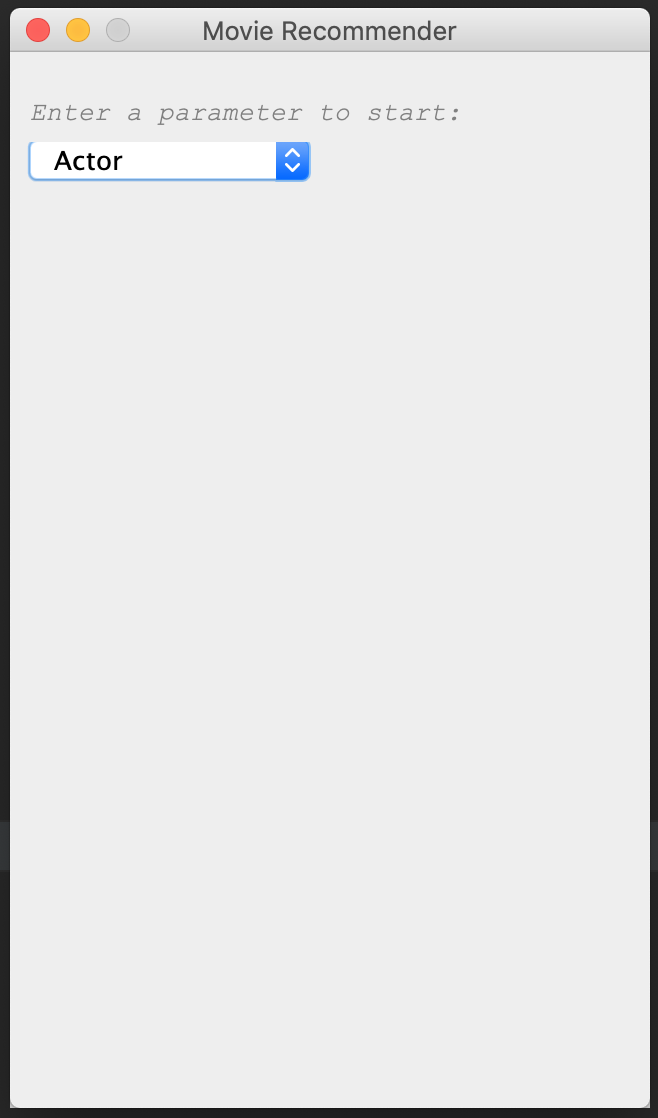
\includegraphics[width=0.5\linewidth]{images/telaInicial1}
 	\caption{Tela Inicial}
 	Fonte: pessoal.
 	\label{fig:Tela Inicial}
 \end{figure}
 
 \begin{figure}[H]
 	\centering
 	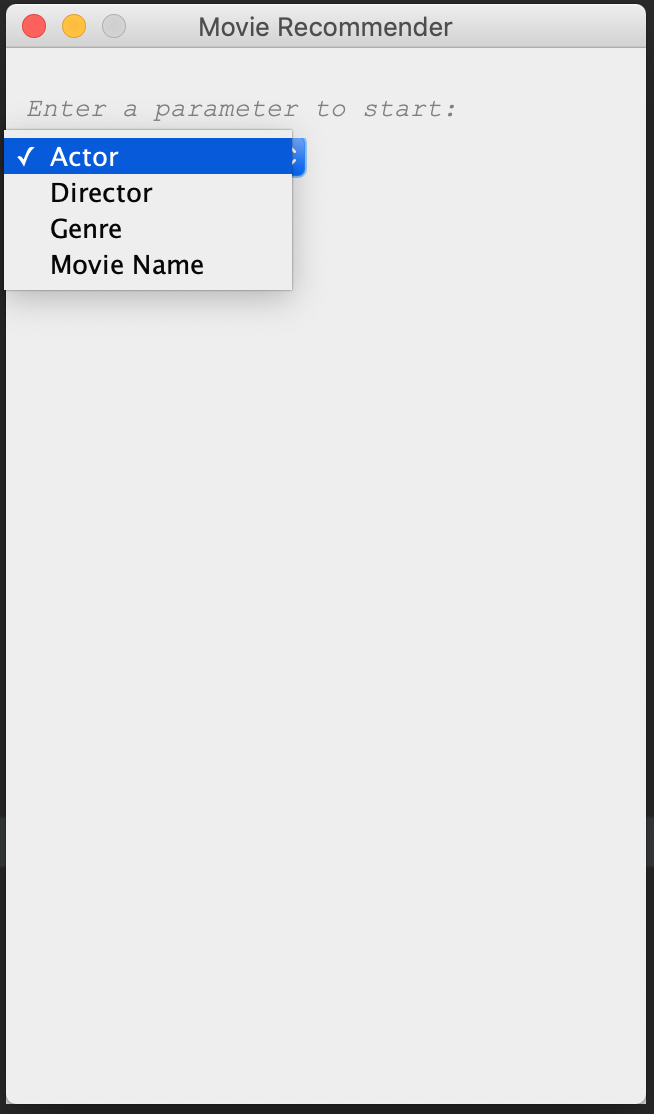
\includegraphics[width=0.5\linewidth]{images/telaInicial2}
 	\caption{Tela Inicial}
 	Fonte: pessoal.
 	\label{fig:Tela Inicial}
 \end{figure}

\subsection{Parâmetro de Entrada} 

 Tendo o usuário selecionado o primeiro parâmetro, é necessário informar o parâmetro de entrada que será usado na query para trazer as informações correspondentes.
 
 No exemplo (Figura 3), optou-se pelo parâmetro inicial ''Actor'' e parâmetro de entrada igual a ''Leonardo DiCaprio''.
 
  \begin{figure}[H]
 	\centering
 	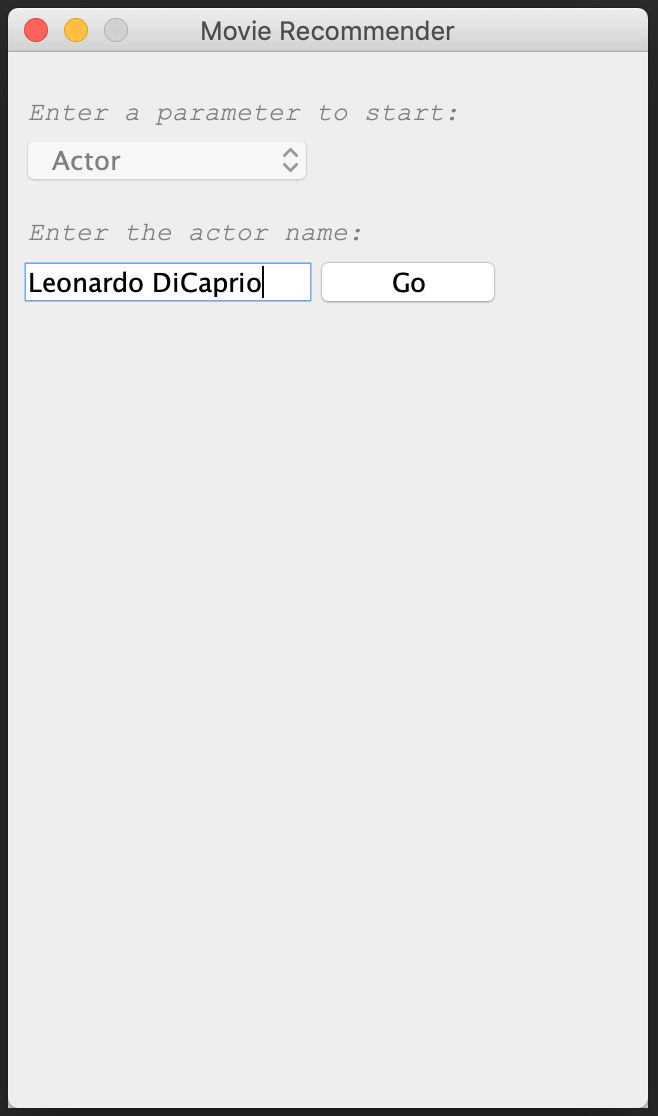
\includegraphics[width=0.5\linewidth]{images/telaInicialPreenchida}
 	\caption{Tela Inicial Preenchida}
 	Fonte: pessoal.
 	\label{fig:Tela Inicial Preenchida}
 \end{figure}

 Evidentemente, ao pressionar o botão ''Go'' a query será executada e as informações existentes na base de dados RDF serão trazidas para a tela em formato de recomendação (Figura 4).
 
   \begin{figure}[H]
 	\centering
 	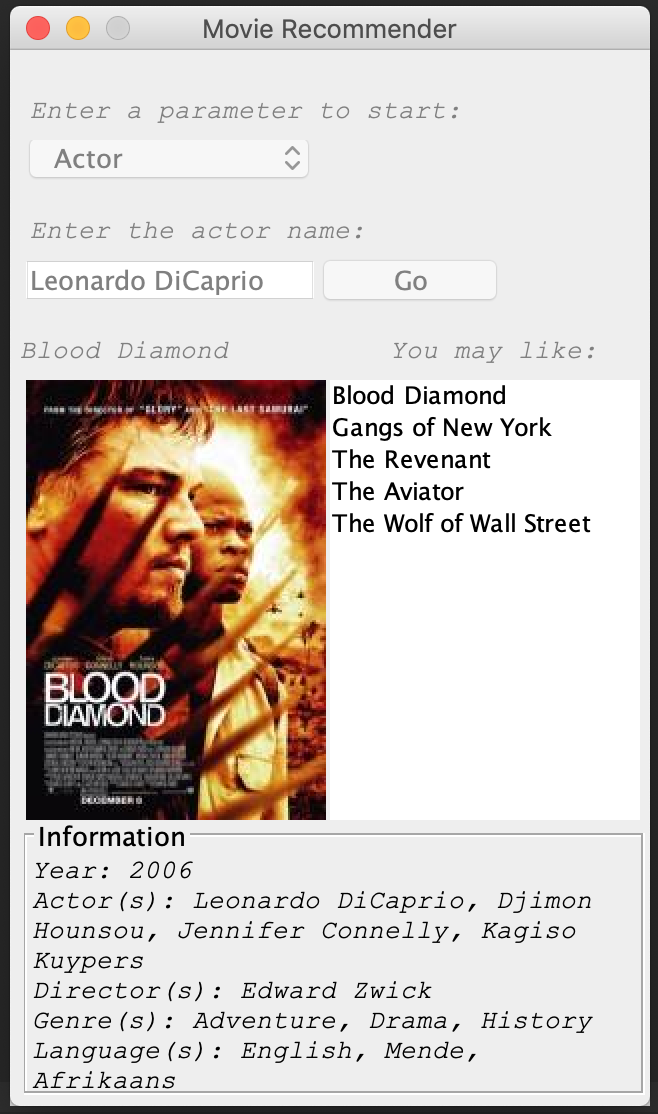
\includegraphics[width=0.5\linewidth]{images/telaInicialRecomendacao}
 	\caption{Tela Inicial com Recomendações}
 	Fonte: pessoal.
 	\label{fig:Tela Inicial com Recomendações}
 \end{figure}


\subsection{Funcionalidades e Navegação} 
 
 Uma vez que a pesquisa foi realizada com sucesso, o usuário encontra à esquerda o pôster, à direita as recomendações equivalentes aos parâmetros fornecidos e abaixo informações pertinentes ao filme.
 
 O usuário tem liberdade de escolher outro filme na sessão ''You may like'', alterando, evidentemente, as informações exibidas (Figura 5).
 
   \begin{figure}[H]
	\centering
	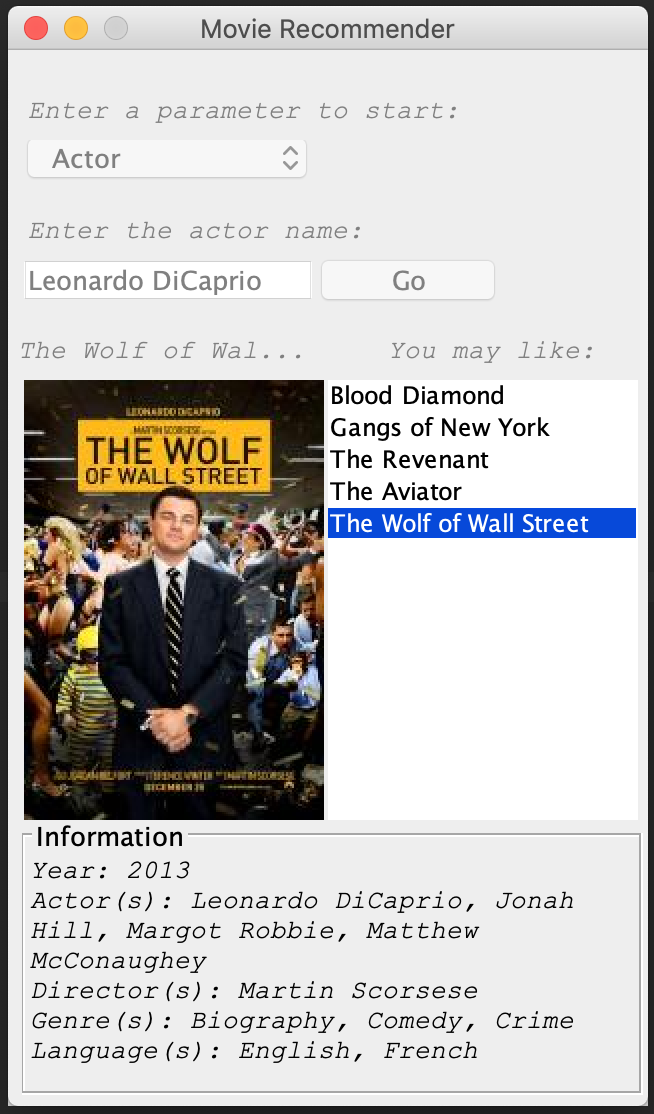
\includegraphics[width=0.5\linewidth]{images/telaInicialRecomendacao2}
	\caption{Tela Inicial alternando Recomendações}
	Fonte: pessoal.
	\label{fig:Tela Inicial alternando Recomendações}
\end{figure}
 
 A aplicação ainda prevê o encaminhamento para a crítica do filme pelo jornal estadunidense The New York Times, se existente, por intermédio do clique do mouse no pôster (Figura 6).
 
   \begin{figure}[H]
	\centering
	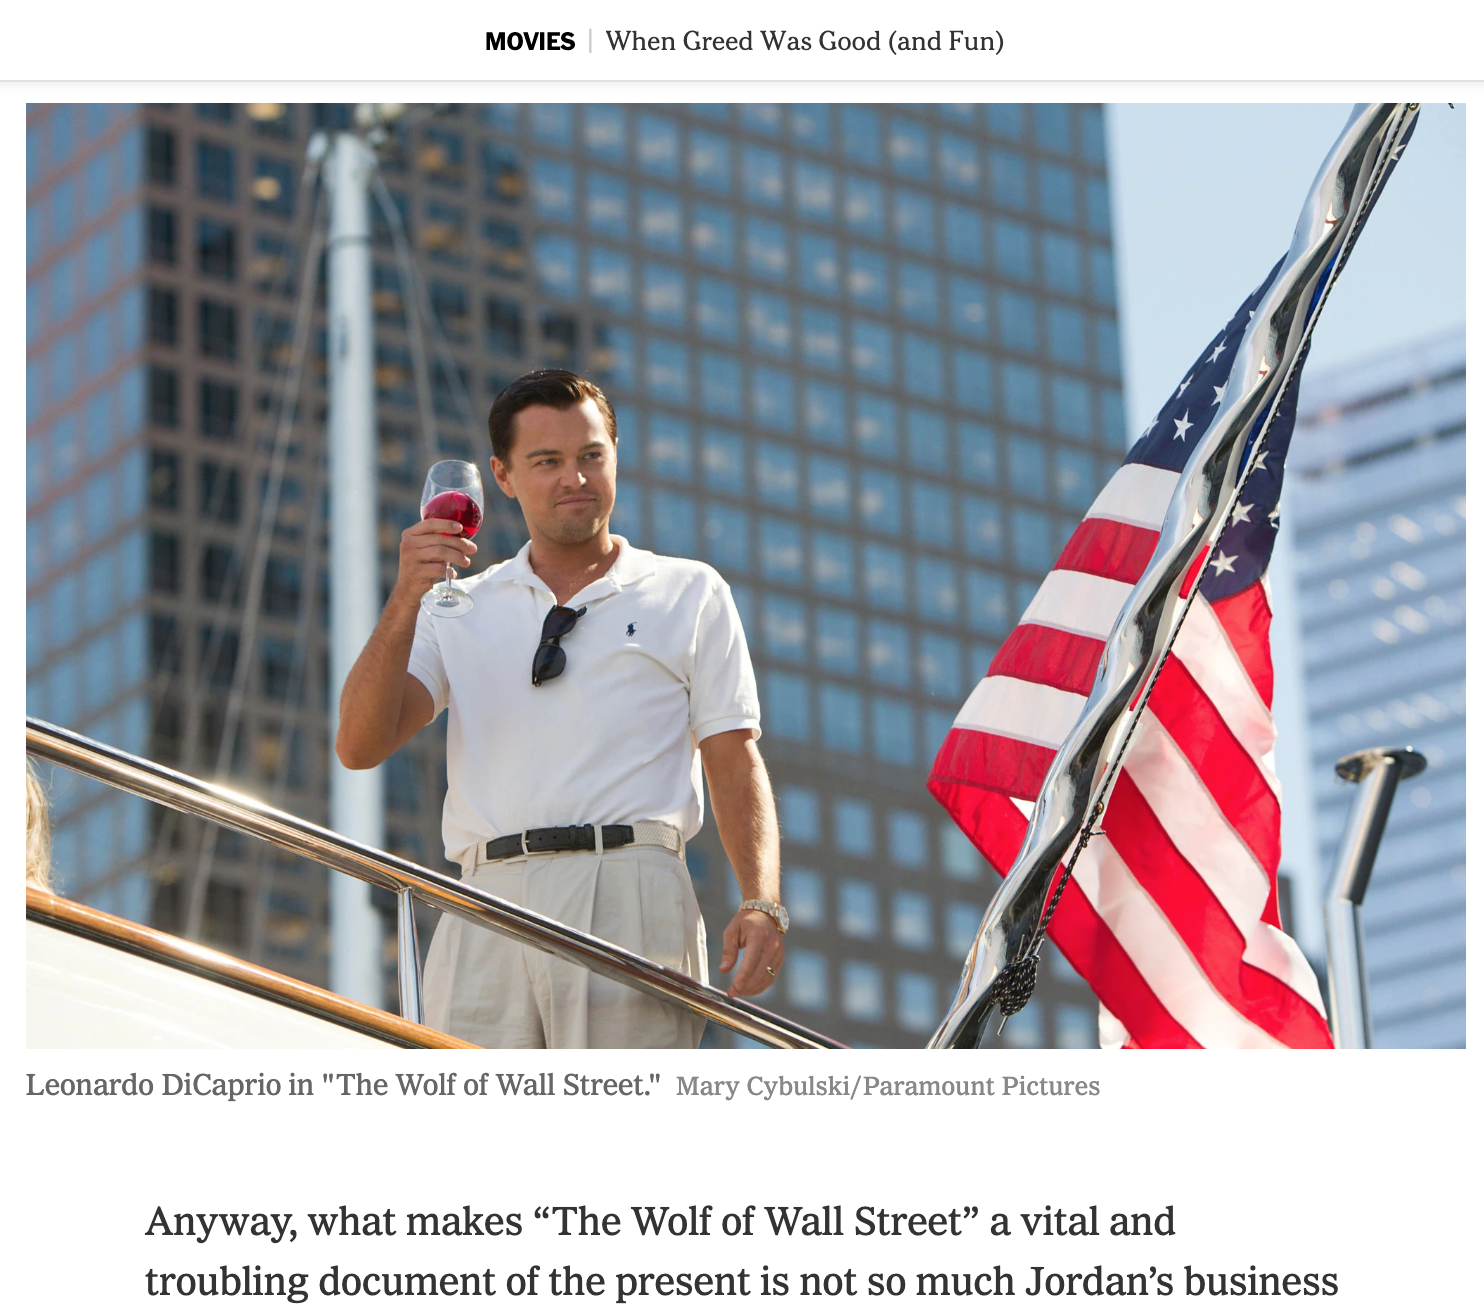
\includegraphics[width=0.6\linewidth]{images/NYTIMES}
	\caption{Crítica - The New York Times}
	Fonte: pessoal.
	\label{fig:Crítica - The New York Times}
\end{figure}

\section{Consulta/Query}

 As queries buscam, especificamente, o parâmetro de entrada baseado no parâmetro inicial.
 
 No exemplo anterior, utilizou-se o parâmetro inicial ''Actor'' e parâmetro de entrada ''Leonardo DiCaprio''. Dessa forma, a aplicação deve montar a querie seguindo o formato abaixo (Figura 7).

\begin{figure}[H]
	\centering
	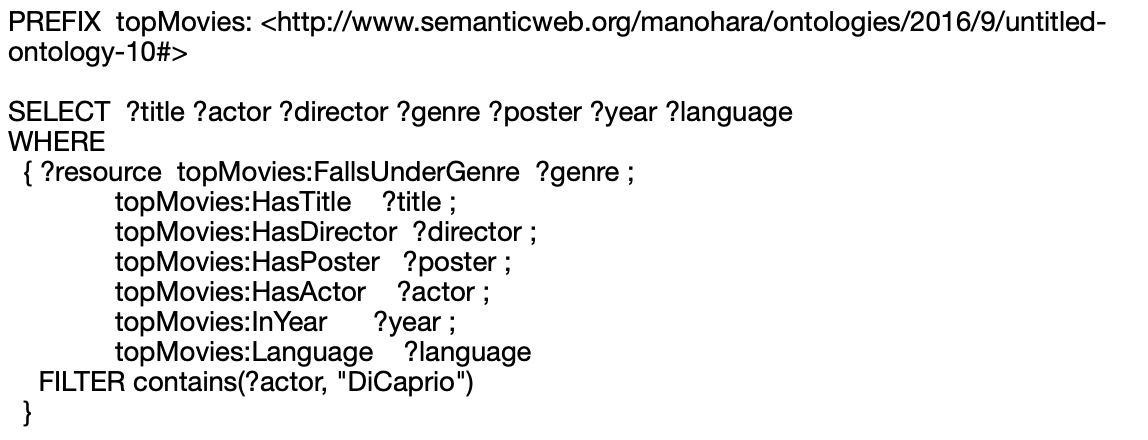
\includegraphics[width=0.8\linewidth]{images/Query}
	\caption{Exemplo de Query}
	Fonte: pessoal.
	\label{fig:Exemplo de Query}
\end{figure}

A manipulação é feita por intermédio da classe ResultSet do Java e permite a atribuição do resultado nas variáveis para exibição.
	\chapter{Tecnologias}\label{cap_tecnologias}

\section{Tecnologias}
Neste trabalho, conforme citado inicialmente, foram usadas as tecnologias de Java, Swing, Jena, GIT e a IDE IntelliJ.

\subsection{Java e Swing}
Dentre estas tecnologias, a linguagem Java foi usada para as telas (especificamente o Swing) e regras de negócio da aplicação. O desenvolvimento em Java só é possível devido às classes para manipulação e execução dos resultados advindos da query, além da própria biblioteca Jena.

\subsection{IDE Intellij}
Também foi utilizada IDE IntelliJ para facilitar o desenvolvimento, "O IDE é um programa de computador, geralmente utilizado para aumentar a produtividade dos desenvolvedores de software, bem como a qualidade desses produtos. Podem auxiliar, através de ferramentas e características, na redução de erros e na aplicação de técnicas como o RAD (Rapid Application Development)".

\subsection{GitHub}
Também foi feito o uso da ferramenta de controle de versão GitHub para gerenciar os arquivos de desenvolvimento e também deste relatório.
	\chapter{Conhecimentos Utilizados aprendidos na disciplina}\label{ch-aula}

\section{Conhecimentos}

A disciplina de Linguagens Comerciais de Programação abordou diversos conceitos da linguaguem Java. Dentre eles conexão cliente e servidor, coleções, classes, tipos, Swing para desenvolvimento das telas, threads, banco de dados, etc.
	\chapter{Conclusão}\label{cap_conclu}

Conforme exposto na seção anterior, utilizou-se dos conhecimentos lecionados pela professora Simone das Graças Domingues Prado durante o primeiro semetre de dois mil e dezenove para realização da aplicação que visa permitir a consulta de pagamentos pendentes e controle de matrícula dos alunos de uma academia. Além disso, para o desenvolvimento foi necessário o conhecimento e aprendizado de outras tecnologias não abordadas em aula, mas que complementam o conteúdo como Spring, MongoDB e GIT.

Os realizadores deste projeto acreditam ter aplicado os conhecimentos passados em aula e realizado um projeto pertinente ao proposto.

Também foi possíveis perceber que é totalmente viável um desenvolvimento de um software que possa atender a todos os tipos de academias.

	
	
	% ----------------------------------------------------------
	% Finaliza a parte no bookmark do PDF
	% para que se inicie o bookmark na raiz
	% e adiciona espaço de parte no Sumário
	% ----------------------------------------------------------
	\phantompart
	
	%\chapter{Conclusão}
	
	
	% ----------------------------------------------------------
	% ELEMENTOS PÓS-TEXTUAIS
	% ----------------------------------------------------------
	\postextual
	% ----------------------------------------------------------
	
	% ----------------------------------------------------------
	% Referências bibliográficas
	% ----------------------------------------------------------
	
\end{document}
